\chapter{Introduction}
Data Security can be achieved using information flow policies. Execution of any action
like copying of file, read operation on file or memory, write operation on file or memory, execution of statement etc may cause flow of information. Usually, information revealed that was
unknown before execution of statement termed as information flow otherwise if it was known already then there will be no information flow. This thesis focuses on information flow between
variables used in a python program irrespective of the amount of information flowing. There are two kinds of information flow among variables:\\
\begin{enumerate}
	\item{\textbf{Explicit Information Flow}}\\
   \begin{lstlisting}[language=Python, caption=Python example]
   x = y
   x = math.log(y)\end{lstlisting}
	these assignment operations are example of explicit flow because information related to variable y is flowing into x using data dependency in both cases.
	\item{\textbf{Implicit Information Flow}}\\
	\begin{lstlisting}[language=Python, caption=Python example]
	if y == 1:
		x = 1
	\end{lstlisting}
	\pagebreak
	\begin{lstlisting}[language=Python, caption=Python example, label=lst:whilecode]
	while y < z:
		x = 1
		y += 1\end{lstlisting}
	in these examples value of x after execution of statements depends on the control path
	taken by the program, variable y and z used in choosing between two control path in while
	program, this involvement of y and z in making decision reduce the uncertainty of variables
	y and z. Whether y < z or y > z can be observed with help of final value of x after execution of given code in listing \ref{lst:whilecode} . So there is indirect implicit flow from y to x in the first example and implicit flow from y
	and z to x in the second example\cite{denning}.\\~\\
	\begin{lstlisting}[language=Python, caption=Python example, label=lst:infwhile]
	x = 0
	while y == 1:
		pass
	x = 1\end{lstlisting}
   Here assignment operation on x in Listing \ref{lst:infwhile} is outside of while body but still information flowing from y to x because execution of x = 1 statement depends on termination of while loop, so you can know value of y by checking the value of x after execution of program, for example if value of x is 1 and program terminated then y must be other than 1, if while loop goes in infinite loop then y must be 1.
   
   The first chapter describes python program certification with the help of Denning's Lattice Model. The lowest security class in this lattice assumed is Low everyone can read information from this class, the highest class in the lattice is High, 
   information from all security classes can flow into it but no information can flow from this class to others.
For Example certification of python code in Listing \ref{lst:lattice} needs to follow Denning's lattice and constraints written in figure \ref{fig:lattice}, security class of variable var is denoted by \dud{var}.  
	\begin{lstlisting}[language=Python,caption={Python example}, label={lst:lattice}]
	x = 0
	z = 1
	y = 0
	if x :
		while z :
			y = 1\end{lstlisting}
	\begin{figure*}[h]
		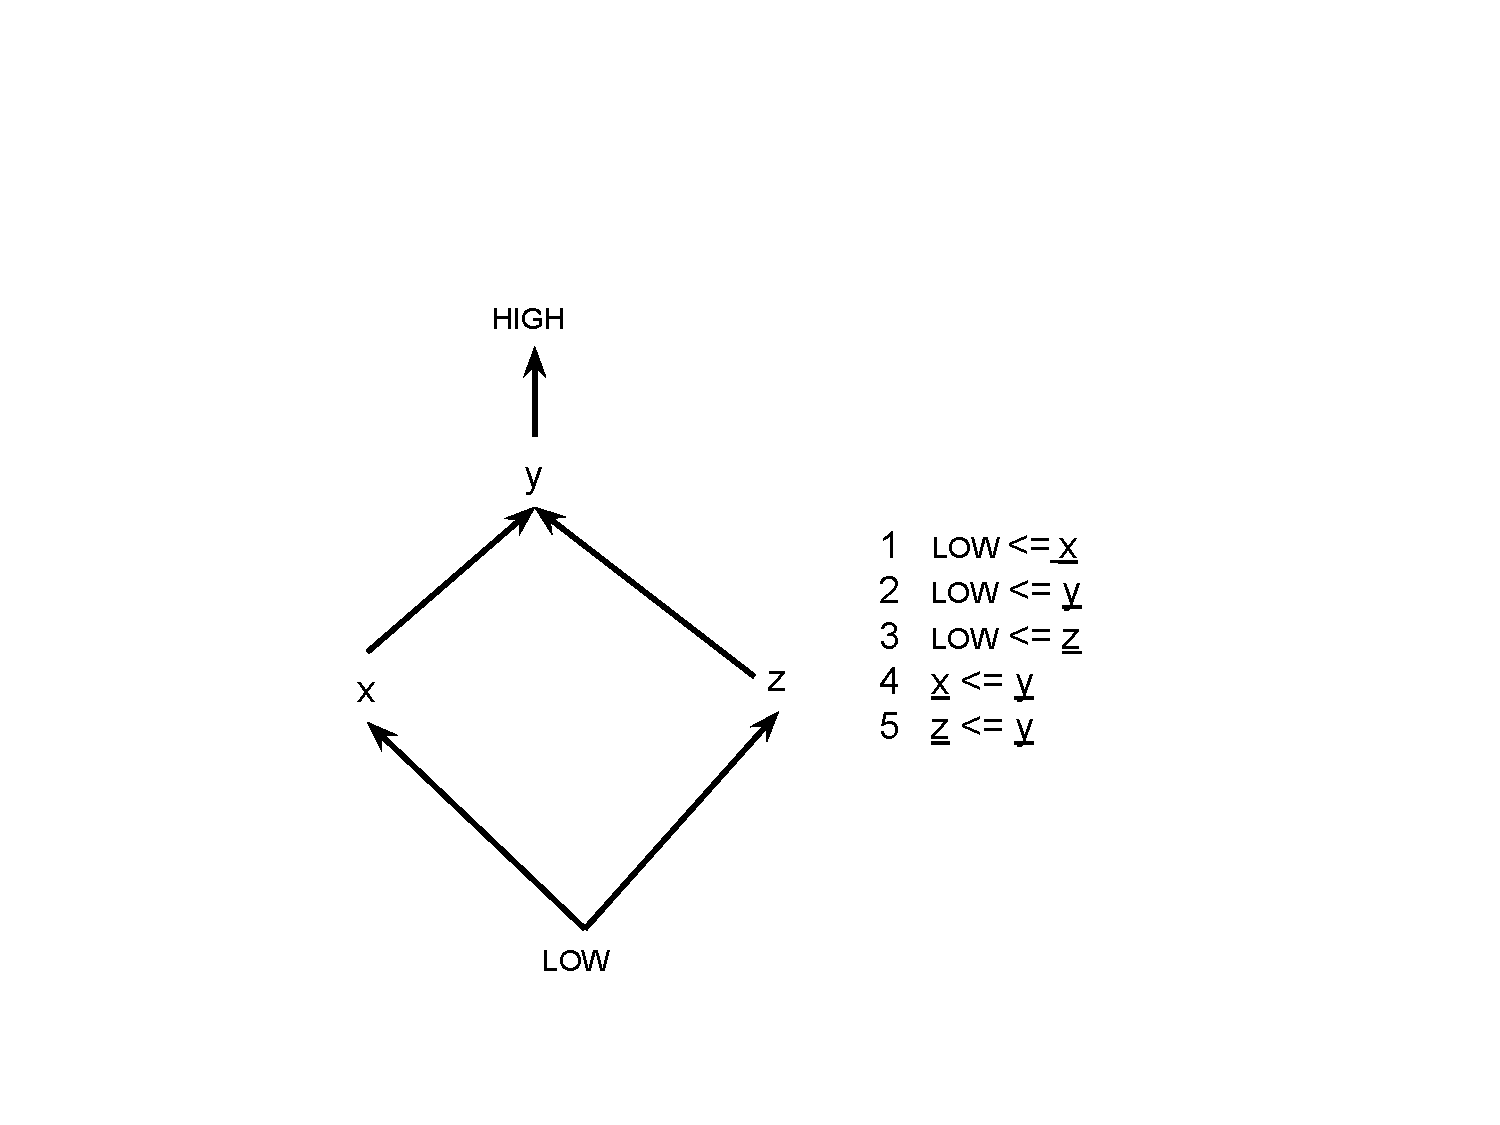
\includegraphics[width=0.6\textwidth]{lattice}
		\centering
		\caption{Lattice of Listing \ref{lst:lattice}}
		\label{fig:lattice}
	\end{figure*}
    Chapter \ref{ch:denning} describes information flow by nonterminating while loop and how to certify program in such situation.
    Chapter \ref{ch:thread} describes how information flows among thread in the multi-threaded program using semaphore.
    Chapter \ref{ch:label} presents a new approach to certifying a program using more sophisticated labels (RWFM label)
    and it also considers subjects for certification of the program.	
\end{enumerate}     

\section{Motivation}
In the field of data security, there are a lot of approaches to prevent leak of information for example cryptography takes care of confidentiality and integrity while data is transmitting through less secure networks, access permission on files prevent unauthorized access to files in a system where users have different privileges. But at the time of execution of program, data used in the program is vulnerable to various attacks so to maintain security at the time of execution of program and processing of data, information flow policies are used. The subject is defined as an executing authority it can be a user or parent process, object can be a file, program variable, memory location etc. In a multilevel security system a subject has permission related to objects. Information flow verification of program only considering objects may seem to be secure but with a particular subject same program may be insecure, so we considered subjects in static analysis of python program.   

\section{Goals}
To develop a platform that takes input a python program and labels of each variable used in the program, and provide answers to various queries regarding the security of information flow.   

\section{Contributions}
\begin{figure}
	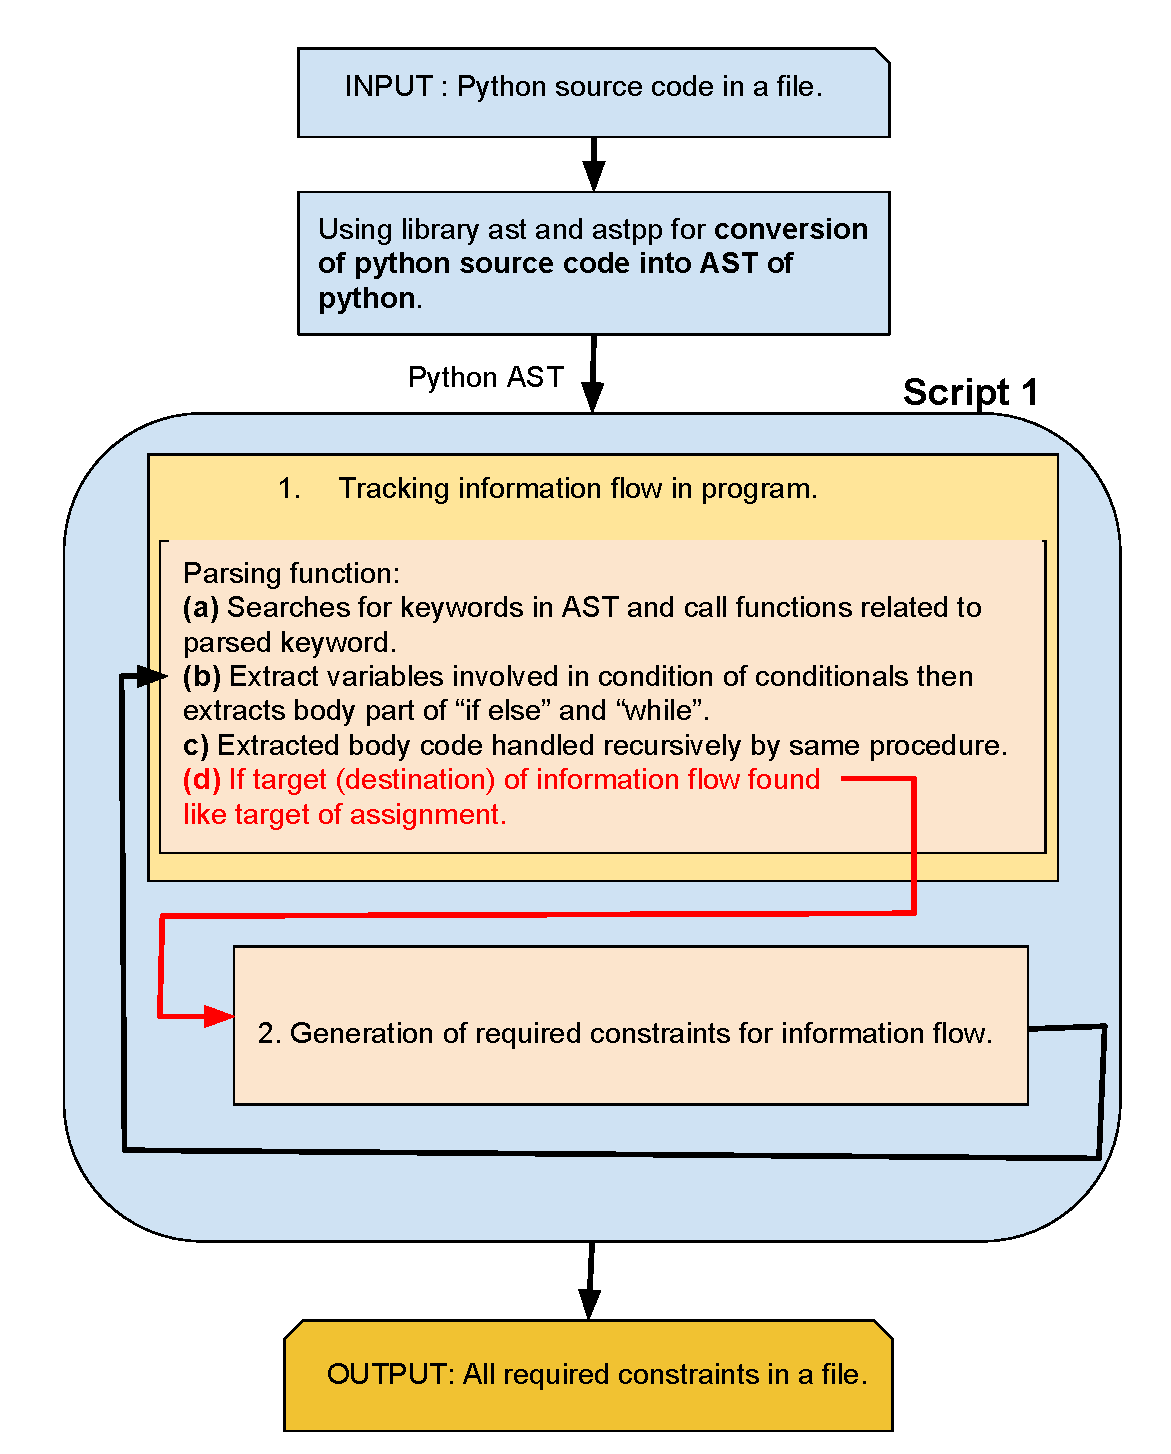
\includegraphics[width=0.6\textwidth]{constraint_gen.pdf}
	\centering
	\caption{Block diagram of script1}
	\label{fig:script1}
\end{figure}
Subject considered with objects for certification of python program. Reader Writer Flow Model \cite{rwfm} used to verify information flows in python program.
\subsection{Implementation Details}
\textbf{Prerequisite Third Party libraries:}
\begin{enumerate}
	\item ast python library (for conversion of python source code into abstract syntax tree)
	\item astpp python library (for readability of of abstract syntax tree of python source code)
\end{enumerate}
\subsubsection{\textbf{Subset of features of python language considered for analysis.}}
\begin{itemize}
	\item Assignment operations : x = e (expression)
	\item Conditional statements : "if else", "elif". \item Iteration : "while".
	\item Semaphore operations : set(), wait(), clear(), initialization of semaphore.
	\item Global variables and local variable in a function.
	\item Function calls and definitions.
	\item Return Statement.	 
\end{itemize}
I implemented fully automated certification platform for python source code  using two python scripts, given in Appendix \ref{ch:script1} and \ref{ch:script2}. Block diagram in figure \ref{fig:script1} shows modules of script1, first python source code is converted into abstract syntax tree (AST) with the help of ast library. The purpose of this step is to avoid tedious work of parsing of source code and comments. Figure \ref{fig:parsing} shows that parsing function reads AST word by word. If function finds any desired word it calls other handler functions to handle code related to particular word, for example: if "While" word is found, parsing function parses body of while and passes it as argument to while\_handler(while\_code) function. Handler function parses variables used in condition and passes the body part to parsing function again. Whenever parsing function finds assignment operation it generates constraint and goes to next word.     
\begin{figure}
	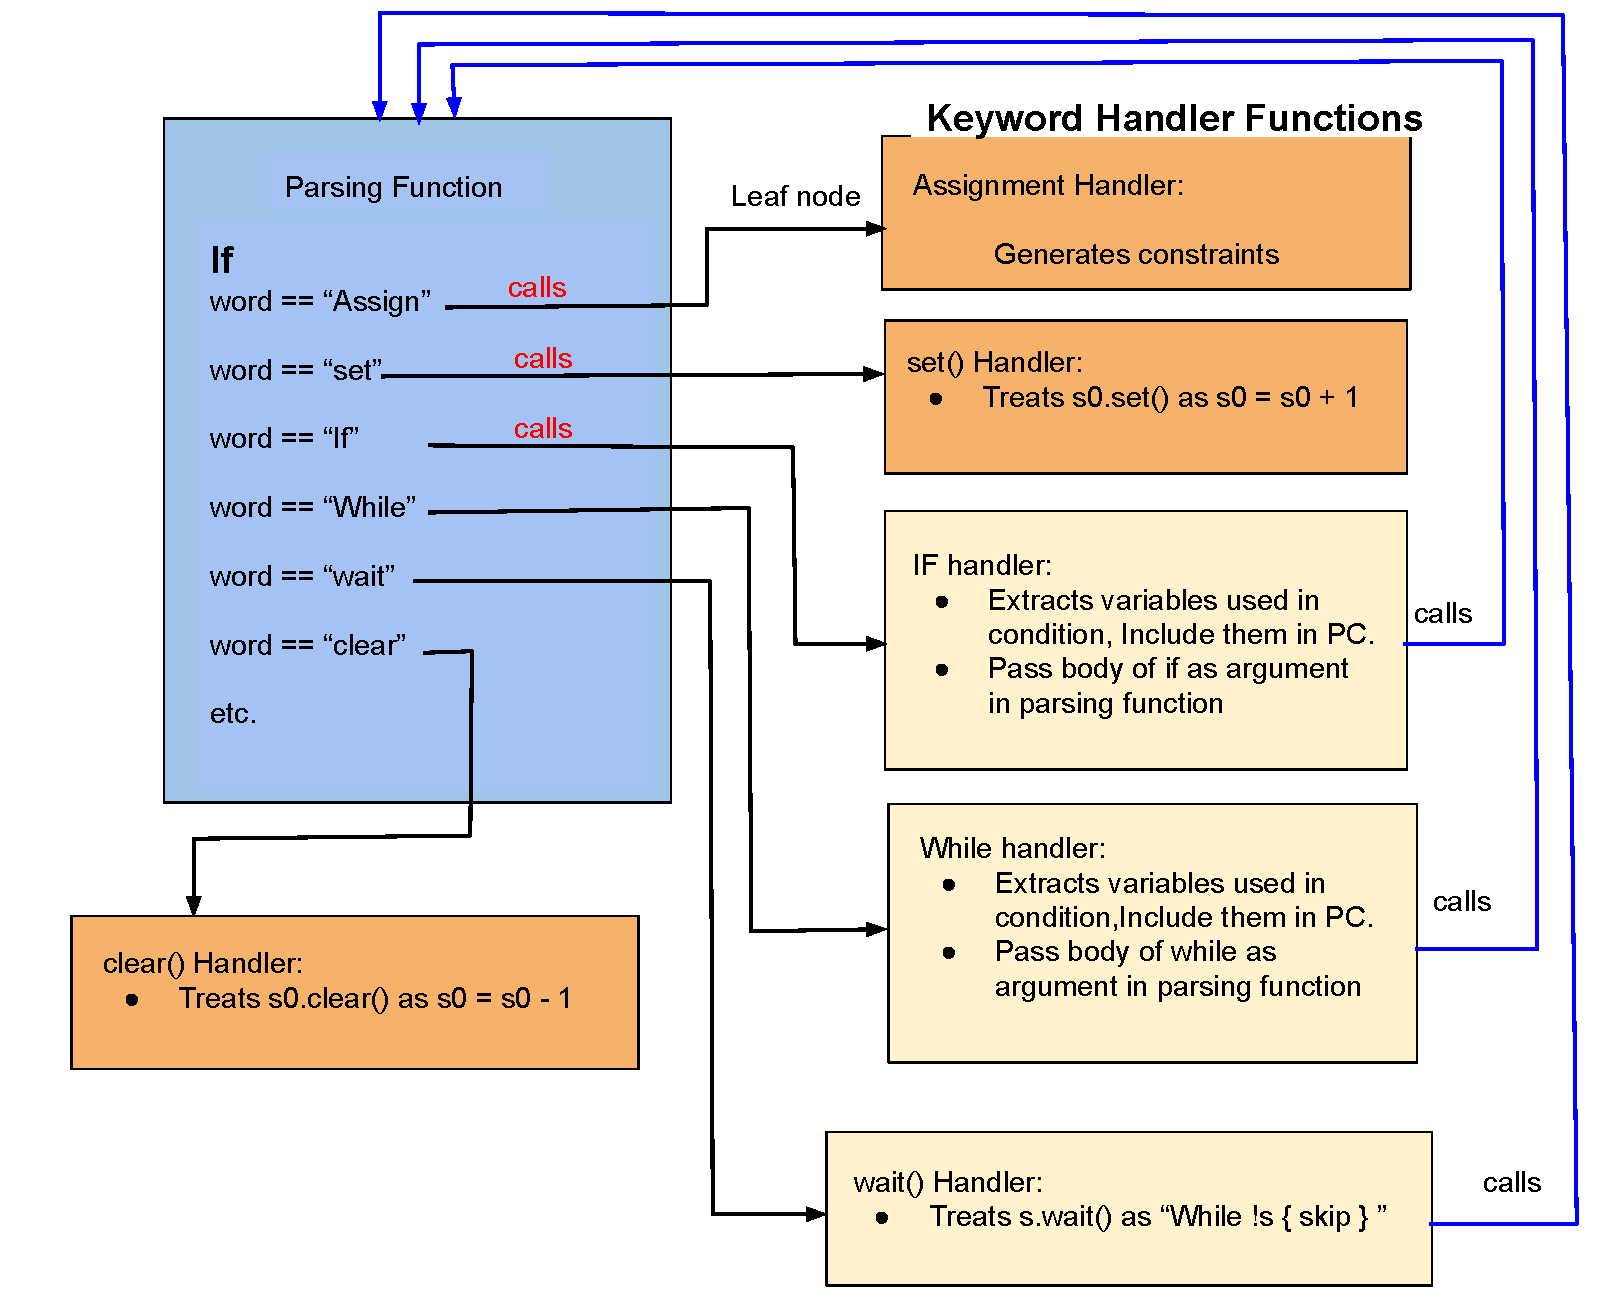
\includegraphics[width=1\textwidth]{parsing.pdf}
	\centering
	\caption{Block diagram of parsing function}
	\label{fig:parsing}
\end{figure}
The Block diagram for script 2 is given in figure \ref{fig:script2} of chapter \ref{ch:label}. 
Effectiveness of this platform depends on the phase of constraint generation because if constraint generator fails to track information flow properly then verifier can not produce correct results. Chapter \ref{ch:c1} to \ref{ch:c4} describe about different constraint generators. Chapter \ref{ch:comp} shows the comparison among all constraint generator.  